\subsection{مقدمه}
برای تست برنامه‌های
\lr{MySQL} و \lr{PostgreSQL}
ما تصمیم گرفتیم که از برنامه‌ی
\link{https://www.hammerdb.com/}{HammerDB}
استفاده کنیم. این برنامه با ساختن دیتابیس‌های
\lr{mock}
و انداختن لود بر روی آن‌ها می‌تواند از عملکرد دیتابیس را تحت نظر داشته باشد.

برای شروع برنامه را دانلود می‌کنیم و آنرا اجرا می‌کنیم. سپس دو بار بر روی
\lr{PostgreSQL} (یا بعدا \lr{MySQL})
کلیک می‌کنیم. سپس پنجره‌ی شکل
\ref{fig:hammerdb:init:benchmark_options}
باز می‌شود.
\begin{figure}[H]
    \centering
    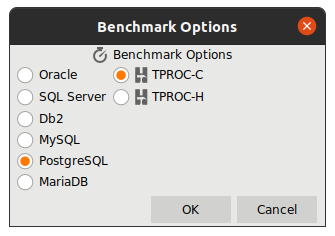
\includegraphics[scale=0.5]{pictures/hammerdb/benchmark-options.png}
    \caption{تنظیمات \lr{benchmark}}
    \label{fig:hammerdb:init:benchmark_options}
\end{figure}
در این پنجره از بین دو نوع
\lr{benchmark}های
\lr{TPROC-C} و \lr{TPROC-H}
می‌توانیم انتخاب کنیم. درباره‌ی فرق این دو در
\link{https://web.archive.org/web/20120919183401/http://www.tpc.org/information/benchmarks.asp}{اینجا}
توضیحات زیادی داده شده است اما به نظر ما و
\link{https://cloud.google.com/compute/docs/tutorials/load-testing-sql-server-hammerdb}{گوگل}
بهتر است که از نوع
C
استفاده کنیم. برای این کار آن را انتخاب می‌کنیم و و منوی آنرا در سمت چپ باز می‌کنیم.
در زیر
\lr{schema}
بر روی
\lr{options}
کلیک می‌کنیم. تنظیمات مورد نظر را انجام می‌دهیم. فعلا
\lr{Number of Workloads}
و
\lr{Virtual Users to Build Schema}
را دست نمی‌زنیم.
\begin{figure}[H]
    \centering
    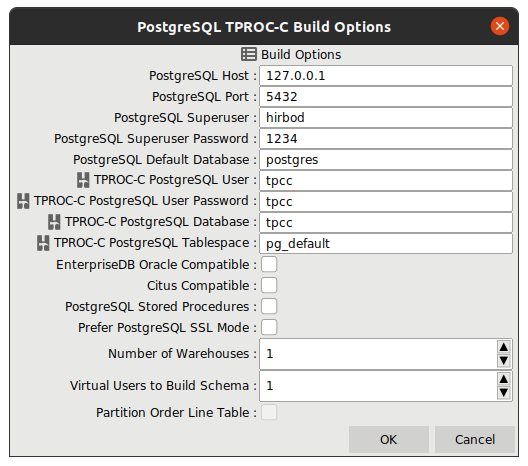
\includegraphics[scale=0.4]{pictures/hammerdb/init.png}
    \caption{تنظیمات دیتابیس}
\end{figure}
سپس بر روی
\lr{build}
کیک می‌کنیم. در اینجا یک دیتابیس با دیتای ماک ساخته می‌شود. می‌توان دیتا را در
\lr{DBeaver}
دید.
\begin{figure}[H]
    \centering
    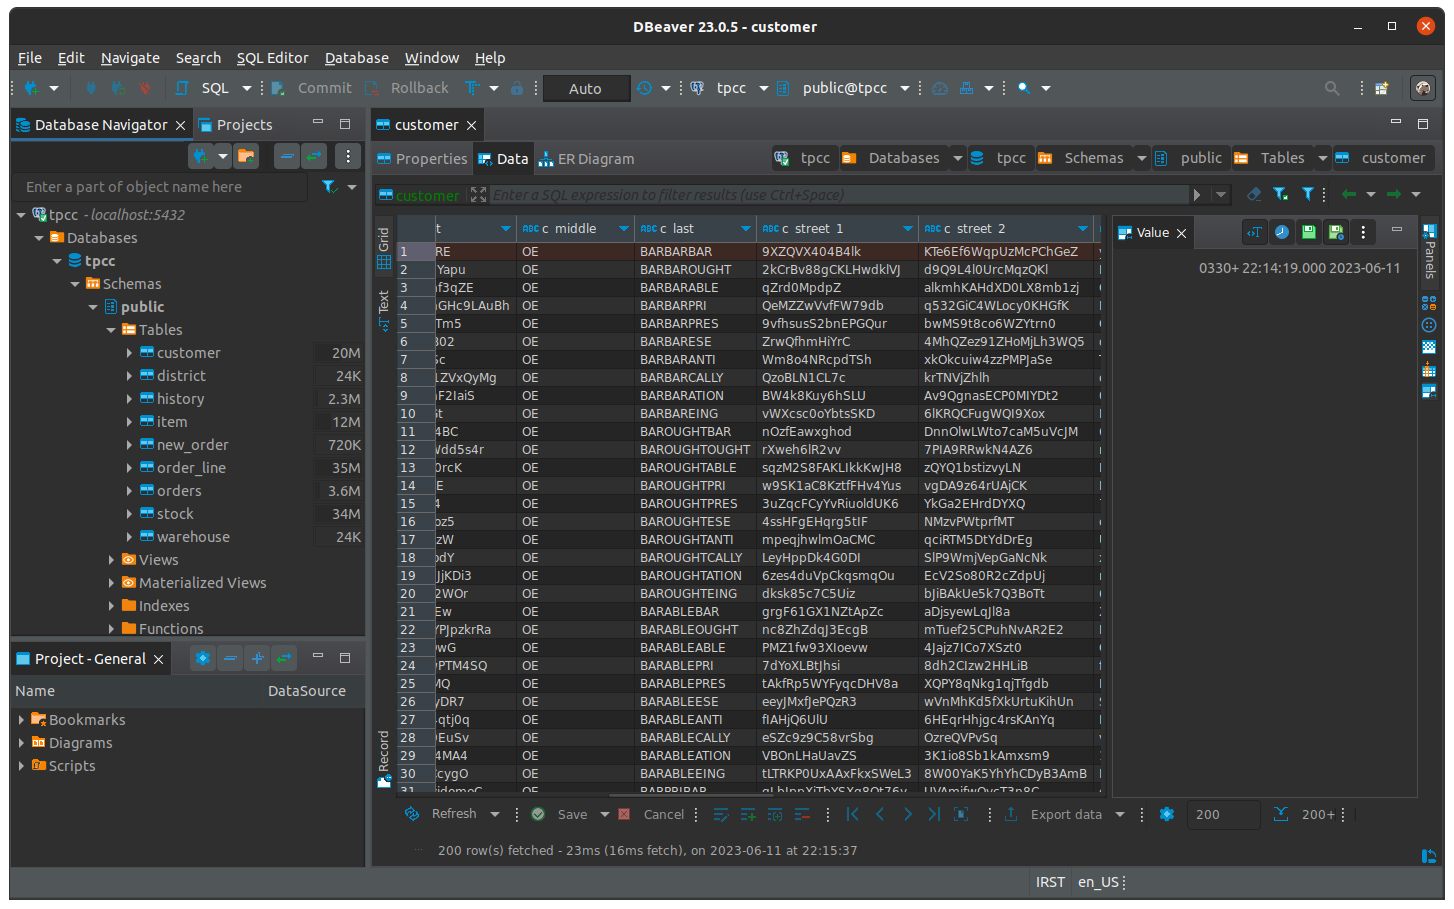
\includegraphics[scale=0.29]{pictures/hammerdb/dbeaver.png}
    \caption{دیتای دیتابیس}
\end{figure}
حال با کلیک کردن دکمه‌ی
\lr{stop}
در بالا عملیات وارد کردن دیتای
\lr{mock}
را متوقف می‌کنیم. سپس در قسمت
\lr{Driver Script}
قسمت
\lr{options}
را انتخاب می‌کنیم. تنظیمات پیش فرض به صورت شکل
\ref{fig:hammerdb:init:default_driver}
هستند.
\begin{figure}[H]
    \centering
    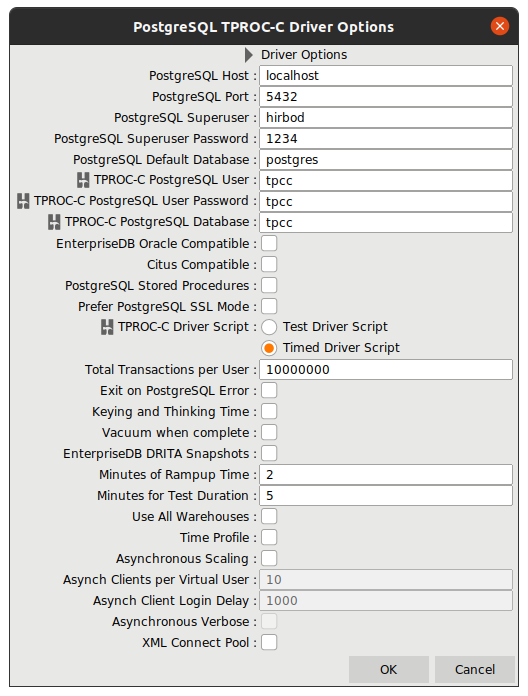
\includegraphics[scale=0.5]{pictures/hammerdb/default-driver.png}
    \caption{تنظیمات درایور}
    \label{fig:hammerdb:init:default_driver}
\end{figure}
برای یک تست نمونه این تنظیمات را دست نمی‌زنیم و صرفا همین را تایید می‌کنیم. حال با دو بار کلیک کردن بر روی دکمه‌ی
\lr{load}
اسکریپت بنچمارک لود می‌شود. سپس در منوی
\lr{autopilot}،
آنرا فعال می‌کنیم و بر روی دکمه‌ی
\lr{autopilot}
می‌زنیم. با این کار تست شروع می‌شود. همان طور که مشخص است
\lr{btop}
مصرف بالای دیسک را نشان می‌دهد که از
\lr{PostgreSQL}
است. به عنوان
\lr{side note}
نیز باید ذکر کنم که
\lr{autopilot}
چندین تست با چندین تعداد فعال همزمان بر روی دیتابس می‌گیرد.

\begin{figure}[H]
    \centering
    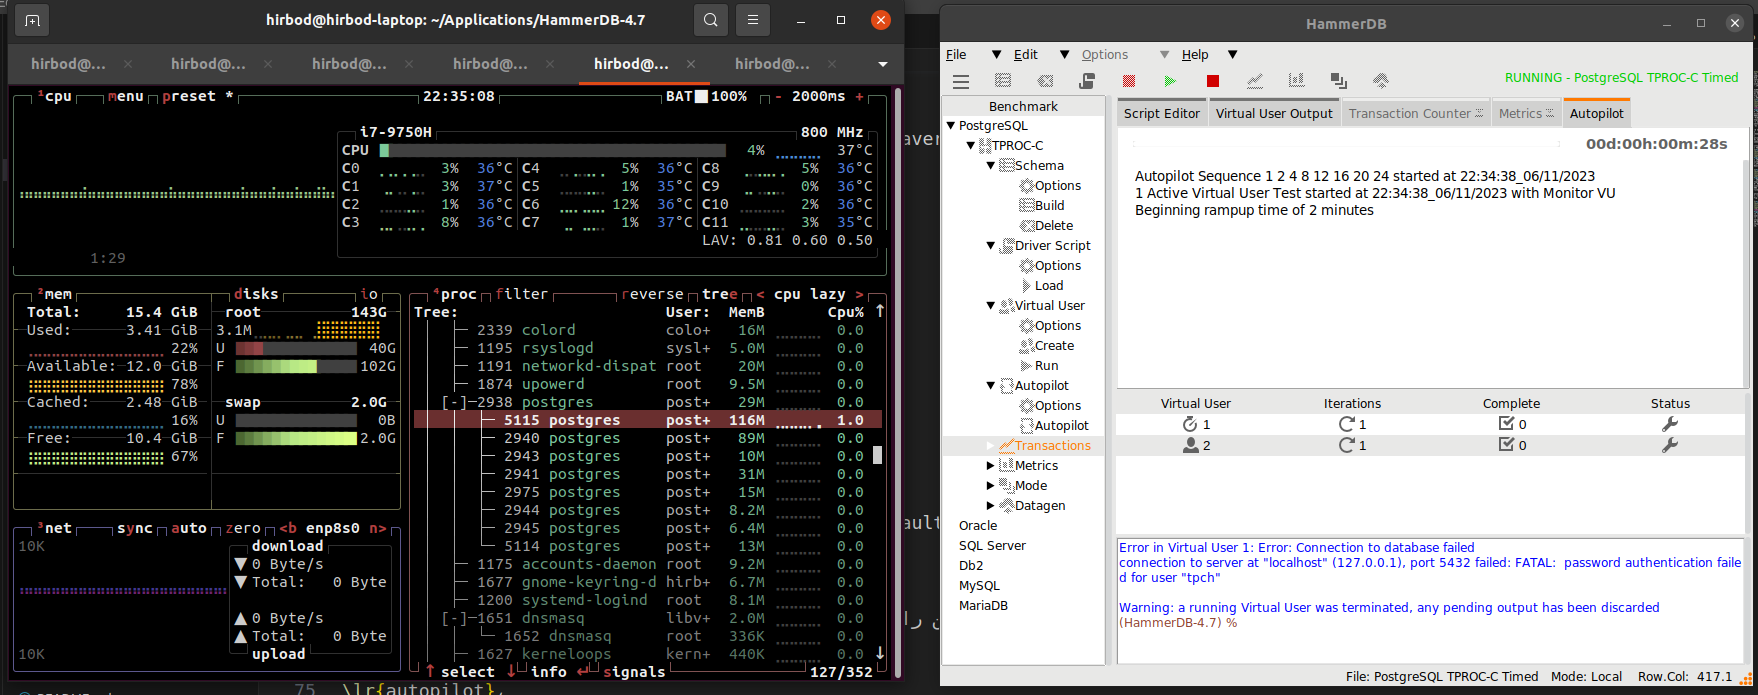
\includegraphics[scale=0.23]{pictures/hammerdb/sample-run.png}
    \caption{\lr{HammerDB + btop}}
\end{figure}

در نهایت زمانی که کارمان تمام شد نیز بر روی
\lr{delete schema}
کلیک می‌کنیم که دیتابیس پاک شود.